\section{PRISMA: Projection of Representations for Interpretability
Sparse Monosemantic Autoencoders}

\begin{figure}[htbp]
    \centering
    \includegraphics[width=\textwidth]{pictures/cap5/home.png}
    \caption{Home page di PRISMA}
    \label{fig:prisma_home}
\end{figure}

\subsection{Fare luce nella black box degli embeddings}
\label{sec:prisma_intro}
Nel capitolo precedente abbiamo identificato i due ostacoli fondamentali che impediscono di interpretare le rappresentazioni neurali: l'opacità—non conosciamo le direzioni $\mathbf{w}_i$ lungo cui sono codificate le feature—e l'interferenza—anche conoscendole, non potremmo recuperare le intensità $a_i$ in modo pulito a causa della non-ortogonalità. Abbiamo anche delineato una via d'uscita teorica: espandere lo spazio delle rappresentazioni e imporre sparsità, così da forzare ogni feature a occupare un asse dedicato.
Questo capitolo presenta PRISMA, un'applicazione sviluppata in questa tesi che implementa concretamente questa strategia. Il nome non è casuale: richiama l'analogia con il prisma ottico, uno strumento che non genera luce, ma la scompone. Quando un fascio di luce bianca attraversa un prisma, ne emergono le componenti spettrali—rosso, arancione, giallo, e così via—che erano già presenti nel fascio originario, ma indistinguibili a occhio nudo. Il prisma non aggiunge informazione: la rende visibile, separando ciò che era mescolato.
\begin{figure}[htbp]
    \centering
    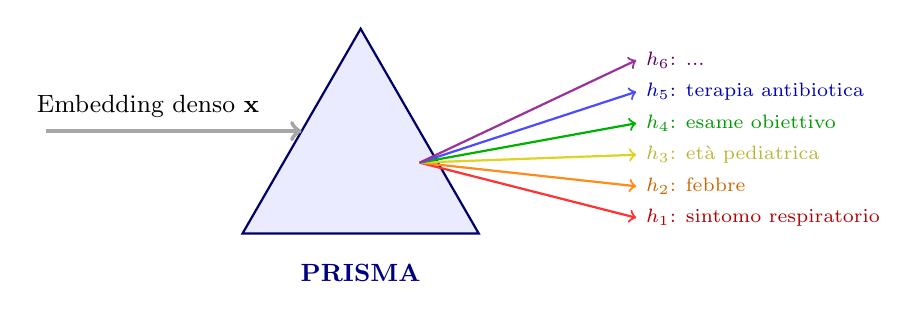
\begin{tikzpicture}[scale=1.0]
        % Prisma (triangolo)
        \coordinate (A) at (0, 0);
        \coordinate (B) at (3, 0);
        \coordinate (C) at (1.5, 2.6);
        
        \fill[blue!8] (A) -- (B) -- (C) -- cycle;
        \draw[thick, blue!40!black] (A) -- (B) -- (C) -- cycle;
        
        % Raggio incidente (bianco/grigio)
        \draw[->, ultra thick, gray!70] (-2.5, 1.3) -- (0.75, 1.3);
        \node[above, font=\small] at (-1.2, 1.35) {Embedding denso $\mathbf{x}$};
        
        % Raggi rifratti (spettro) - escono dal lato destro del prisma
        \draw[->, thick, red!80] (2.25, 0.9) -- (5, 0.2);
        \draw[->, thick, orange!90] (2.25, 0.9) -- (5, 0.6);
        \draw[->, thick, yellow!85!black] (2.25, 0.9) -- (5, 1.0);
        \draw[->, thick, green!70!black] (2.25, 0.9) -- (5, 1.4);
        \draw[->, thick, blue!70] (2.25, 0.9) -- (5, 1.8);
        \draw[->, thick, violet!80] (2.25, 0.9) -- (5, 2.2);
        
        % Etichette feature
        \node[right, font=\scriptsize, red!70!black] at (5, 0.2) {$h_1$: sintomo respiratorio};
        \node[right, font=\scriptsize, orange!80!black] at (5, 0.6) {$h_2$: febbre};
        \node[right, font=\scriptsize, yellow!70!black] at (5, 1.0) {$h_3$: età pediatrica};
        \node[right, font=\scriptsize, green!60!black] at (5, 1.4) {$h_4$: esame obiettivo};
        \node[right, font=\scriptsize, blue!70!black] at (5, 1.8) {$h_5$: terapia antibiotica};
        \node[right, font=\scriptsize, violet!70!black] at (5, 2.2) {$h_6$: ...};
        
        % Etichetta prisma
        \node[font=\small\bfseries, blue!50!black] at (1.5, -0.5) {PRISMA};
        
    \end{tikzpicture}
    \caption{L'analogia ottica di PRISMA. Come un prisma scompone la luce bianca nelle sue componenti spettrali, così PRISMA scompone un embedding denso $\mathbf{x}$ nelle sue feature semantiche costitutive $h_1, h_2, \dots, h_n$. L'informazione era già presente nell'embedding originario, ma codificata in forma opaca; PRISMA la rende esplicita e interpretabile.}
    \label{fig:prisma_analogy}
\end{figure}
PRISMA opera in modo analogo sugli embedding. Un vettore denso $\mathbf{x} \in \mathbb{R}^{768}$, prodotto da un modello come BERT, contiene informazione semantica ricchissima—ma opaca, distribuita su dimensioni che non sappiamo interpretare. PRISMA proietta questo vettore in uno spazio di dimensionalità molto maggiore ($\mathbb{R}^{n}$ con $n \gg 768$), forzando al contempo una rappresentazione sparsa: solo poche componenti $h_i$ possono essere attive per ogni input. Il risultato è una scomposizione in cui ogni componente corrisponde a una feature semantica distinta—un concetto atomico, interpretabile, che possiamo nominare.
L'analogia ha anche una seconda lettura. Il prisma, scomponendo la luce, ci permette di vedere ciò che prima era invisibile. Allo stesso modo, PRISMA fa luce sulla black box degli embedding: non aggiunge capacità predittiva al modello originario, ma rende trasparente ciò che il modello ha appreso. Se la superposition è il meccanismo con cui le reti neurali nascondono la complessità—comprimendo migliaia di concetti in poche centinaia di dimensioni—PRISMA è lo strumento che inverte questo processo, restituendoci una rappresentazione in cui possiamo finalmente leggere quali concetti sono presenti e con quale intensità.
Nel resto di questo capitolo descriveremo l'architettura tecnica che realizza questa scomposizione—lo Sparse Autoencoder—e le metodologie per interpretare automaticamente le feature estratte. Vedremo anche come le feature non siano entità isolate, ma si organizzino in strutture gerarchiche (feature families) e come la loro granularità emerga progressivamente all'aumentare della capacità del modello (feature splitting).